%% 
%% Copyright 2019-2020 Elsevier Ltd
%% 
%% This file is part of the 'CAS Bundle'.
%% --------------------------------------
%% 
%% It may be distributed under the conditions of the LaTeX Project Public
%% License, either version 1.2 of this license or (at your option) any
%% later version.  The latest version of this license is in
%%    http://www.latex-project.org/lppl.txt
%% and version 1.2 or later is part of all distributions of LaTeX
%% version 1999/12/01 or later.
%% 
%% The list of all files belonging to the 'CAS Bundle' is
%% given in the file `manifest.txt'.
%% 
%% Template article for cas-sc documentclass for 
%% double column output.

%\documentclass[a4paper,fleqn,longmktitle]{cas-sc}
\documentclass[a4paper,fleqn]{cas-sc}
\usepackage[utf8]{inputenc}
\usepackage{newunicodechar}
\newunicodechar{₂}{$_2$}
\newunicodechar{₅}{$_5$}

 \usepackage[numbers]{natbib}
%\usepackage[authoryear]{natbib}
%\usepackage[authoryear,longnamesfirst]{natbib}
\usepackage{rotating}%
\usepackage{multirow}%
\usepackage{booktabs}%
\usepackage{graphicx}%
% Overleaf: put PNG/PDF figures in ./figs/ (matches Elsevier convention). Repo also searches figures/ and reports/.
\graphicspath{{figs/}{figures/}{./}{reports/figures/}}
\usepackage{subcaption}
\usepackage{float}%
%%%Author definitions
\def\tsc#1{\csdef{#1}{\textsc{\lowercase{#1}}\xspace}}
\tsc{WGM}
\tsc{QE}
\tsc{EP}
\tsc{PMS}
\tsc{BEC}
\tsc{DE}
%%%

% Uncomment and use as if needed
%\newtheorem{theorem}{Theorem}
%\newtheorem{lemma}[theorem]{Lemma}
%\newdefinition{rmk}{Remark}
%\newproof{pf}{Proof}
%\newproof{pot}{Proof of Theorem \ref{thm}}

\begin{document}
\let\WriteBookmarks\relax
\def\floatpagepagefraction{1}
\def\textpagefraction{.001}

% Short title
\shorttitle{Multi-Horizon Machine Learning Forecasting}

% Short author
\shortauthors{JB Diekuu et~al.}

% Main title of the paper
\title [mode = title]{Multi-Horizon Forecasting of Urban PM$_{2.5}$ Using Attention-Enhanced Deep Learning: Evidence from Coastal Ghana}                      
% Title footnote mark
% eg: \tnotemark[1]
% \tnotemark[1,2]

% Title footnote 1.
% eg: \tnotetext[1]{Title footnote text}
% \tnotetext[<tnote number>]{<tnote text>} 
%\tnotetext[1]{This document is the results of the research project funded by the National Science Foundation.}

% \tnotetext[2]{The second title footnote which is a longer text matter
%    to fill through the whole text width and overflow into
%    another line in the footnotes area of the first page.}


% First author
%
% Options: Use if required
% eg: \author[1,3]{Author Name}[type=editor,
%       style=chinese,
%       auid=000,
%       bioid=1,
%       prefix=Sir,
%       orcid=0000-0000-0000-0000,
%       facebook=<facebook id>,
%       twitter=<twitter id>,
%       linkedin=<linkedin id>,
%       gplus=<gplus id>]
\author[]{John-Bosco Diekuu}
                        %[type=editor,
                        %auid=000,bioid=1,
                        %prefix=Sir,
                        %role=Researcher,
                        %orcid=0000-0001-7511-2910]

% Corresponding author indication
\cormark[1]

% Footnote of the first author
%\fnmark[1]

% Email id of the first author
\ead{j.diekuu@rgu.ac.uk}

% URL of the first author
%\ead[url]{www.cvr.cc, cvr@sayahna.org}

%  Credit authorship
% \credit{Conceptualization, Methodology, Resources,Formal analysis, Data curation, Investigation, Writing - original draft, Writing - review \& editing, Visualization}

% Address/affiliation
\affiliation[1]{organization= {School of Computing}, {Robert Gordon University},
    addressline={Garthdee}, 
    city={Aberdeen},
    % citysep={}, % Uncomment if no comma needed between city and postcode
    postcode={AB10 7GJ}, 
    % state={},
    country={UK}}

% Second author
\author%
%[]
{Ulric Sena Abonie}
%\cormark[2]
%\fnmark[1]
% \ead{ms.mekala@rgu.ac.uk}
%\ead[URL]{www.stmdocs.in}

%\affiliation[3]{organization={STM Document Engineering Pvt Ltd.},
  %  addressline={Mepukada}, 
    %city={Malayinkil},
    % citysep={}, % Uncomment if no comma needed between city and postcode
   % postcode={695571}, 
   % state={Trivandrum},
   % country={India}}
   % \credit{ Writing - review \& editing}
% Address/affiliation
%\affiliation[2]{organization={Sayahna Foundation},
    % addressline={}, 
   % city={Jagathy},
    % citysep={}, % Uncomment if no comma needed between city and postcode
    %postcode={695014}, 
   % state={Trivandrum},
  %  country={India}}

% Fourth author
\author%
%[]
{Prosper K. Yeng}
%\cormark[2]
%\fnmark[1]
% \ead{j.p.isaacs@rgu.ac.uk}
%\ead[URL]{www.stmdocs.in}

%\affiliation[3]{organization={STM Document Engineering Pvt Ltd.},
  %  addressline={Mepukada}, 
    %city={Malayinkil},
    % citysep={}, % Uncomment if no comma needed between city and postcode
   % postcode={695571}, 
   % state={Trivandrum},
   % country={India}}
   % \credit{ Writing - review \& editing}
\author%
%[]
{Eric Kemeh}
%\cormark[2]
%\fnmark[1]
% \ead{j.p.isaacs@rgu.ac.uk}
%\ead[URL]{www.stmdocs.in}

%\affiliation[3]{organization={STM Document Engineering Pvt Ltd.},
  %  addressline={Mepukada}, 
    %city={Malayinkil},
    % citysep={}, % Uncomment if no comma needed between city and postcode
   % postcode={695571}, 
   % state={Trivandrum},
   % country={India}}
   % \credit{ Writing - review \& editing}

   \author[]{Eyad Elyan}

% Third author
%\author[2,3]{CV Rajagopal}[%
  % role=Co-ordinator,
   %suffix=Jr,
  % ]
% \cormark[2]
%\fnmark[1]
% \ead{e.elyan@rgu.ac.uk}
%\ead[URL]{www.sayahna.org}

% \credit{Conceptualization, Methodology, Formal analysis, Investigation, Writing - original draft, Writing - review \& editing, Data curation}


% Corresponding author text
\cortext[cor1]{Corresponding author}
% \cortext[cor2]{Principal corresponding author}


% Footnote text
% \fntext[fn1]{This is the first author footnote. but is common to third
%   author as well.}
% \fntext[fn2]{Another author footnote, this is a very long footnote and
%   it should be a really long footnote. But this footnote is not yet
%   sufficiently long enough to make two lines of footnote text.}

% % For a title note without a number/mark
% \nonumnote{This note has no numbers. In this work we demonstrate $a_b$
%   the formation Y\_1 of a new type of polariton on the interface
%   between a cuprous oxide slab and a polystyrene micro-sphere placed
%   on the slab.
%   }

% Here goes the abstract
\begin{abstract}
Accurate forecasting of fine particulate matter (PM$_{2.5}$) is critical for managing air quality risks in rapidly urbanising cities. This need is particularly acute in data-constrained regions of sub-Saharan Africa. Thus, this study proposes a multi-horizon predictive modelling framework for urban PM$_{2.5}$ using ground-based observations from Tema, coastal Ghana, collected between September 2025 and February 2026.

Exploratory analysis shows strong seasonal intensification. Mean concentrations increased by approximately 4.8~$\mu$g/m$^3$ per month. A statistically significant regime shift occurred during the Harmattan period. To capture nonlinear temporal dynamics, we utilize an attention-enhanced Long Short-Term Memory (LSTM+attention) model. The model performs direct forecasting at 24-hour, 7-day, 14-day, and 28-day horizons. It is benchmarked against seasonal-naïve and regularised autoregressive baselines.

Results indicate that particle density and seasonal time features dominate predictive performance. Meteorological covariates contribute modestly. The proposed deep learning framework delivers substantial out-of-sample improvements over statistical baselines, particularly at medium-term horizons. It remains stable during high-pollution episodes.

These findings demonstrate the value of attention-based sequence modelling for urban air quality forecasting in resource-limited environments. The framework provides an operational basis for early warning and risk-informed air quality management in Ghana.

\end{abstract}



% Use if graphical abstract is present
% \begin{graphicalabstract}
% \includegraphics{figs/grabs.pdf}
% \end{graphicalabstract}

% Research highlights
\begin{highlights}
\item Multi-site hourly PM$_{2.5}$ forecasting in coastal Tema using direct horizons of 24~h through 28~days.
\item Attention-augmented LSTM sequence modelling benchmarked against lag--Fourier baselines and classical machine learning on leakage-safe time splits.
\item Stress-tested performance during Harmattan versus pre-Harmattan conditions and during upper-decile pollution episodes.
\end{highlights}

% Keywords
% Each keyword is seperated by \sep
\begin{keywords}
Urban air quality modelling\sep Multi-horizon prediction\sep PM$_{2.5}$ forecasting\sep Attention-based deep learning
\end{keywords}


\maketitle

\section{Introduction} \label{sec1}

Urban air quality is a defining element of the quality of life and the health of the increasingly urban population of industrial societies \cite{volgyesi2008air}. The increasing population, its automobiles and industries in urban cities pollute the air and degrade the air quality \cite{kang2018air}. Ambient air pollution directly affects respiratory and cardiovascular systems, reduces life expectancy, and undermines everyday function \cite{jia2023effect,zhang2023air}. Fine particulate matter including PM$_{2.5}$ and PM$_{10}$, arising from combustion, dust, and chemical transformations, is particularly harmful because it can contain various poisonous chemicals and be breathed into human lungs. PM$_{2.5}$ is globally recognised as a critical indicator of urban air quality and is commonly used to define national air quality standards \cite{hodoli2024urban}. Elevated PM$_{2.5}$ is associated with increased hospital admissions for asthma, bronchitis and other cardiorespiratory conditions and millions of premature deaths globally each year \cite{lelieveld2019effects,world2021global}. The World Health Organization’s updated air quality guidelines recommend an annual mean PM$_{2.5}$ concentration of 5~$\mu$g/m$^3$, yet most cities exceed this threshold \cite{pai2022updated}. Environmental effects of air pollution include haze, eutrophication, and global climate change \cite{kang2018air}. Air pollution directly undermines the attainment of SDG 3 (Good Health and Well-Being) and SDG 11 (Sustainable Cities and Communities). 

% Urban air quality is a defining element of environmental health in rapidly growing cities. Ambient air is a shared resource; when it degrades, it directly affects respiratory and cardiovascular systems, reduces life expectancy, and undermines everyday function \cite{jia2023effect,zhang2023air}.  Fine particulate matter (PM$_{2.5}$ and PM$_{1.0}$), arising from combustion, dust, and chemical transformations, is particularly harmful because it penetrates deep into the lungs and bloodstream. Exposure to PM$_{2.5}$ has been linked to millions of premature deaths globally each year \cite{world2021global}. The World Health Organization’s updated air quality guidelines recommend an annual mean PM$_{2.5}$ concentration of 5~$\mu$g/m$^3$, yet most cities exceed this threshold \cite{world2021global}. Elevated PM$_{2.5}$ is associated with increased hospital admissions for asthma, bronchitis and other cardiopulmonary conditions \cite{lelieveld2019effects}. Improving air quality contributes directly to SDG~3 (Good Health and Well-Being) and SDG~11 (Sustainable Cities and Communities).
Air pollution has become a pressing problem for developing countries, due to the rapid development in industry and transportation \cite{zheng2016design}. Urban air quality management is dependent on the availability of local air pollution data and the ability to predict future pollution patterns. If air quality continues to deteriorate, the cost of pollution harness may become a heavy burden for governments \cite{zheng2016design}. Thus, air quality monitoring systems are very useful in effectively monitoring air pollution before the situation becomes worse \cite{zheng2016design}. Research in developed countries demonstrates that systematic measurement and policy can improve air quality. In cities in the UK, the introduction of ultra-low emission zones and stricter vehicle standards reduced traffic-related PM$_{2.5}$ and nitrogen dioxide, lowering population exposure \cite{rodrigues2025london}. Similarly, dense monitoring networks in cities such as Tokyo and Los Angeles have enabled real-time air quality forecasting, supporting public health advisories and mitigation strategies \cite{agarwal2025assessing,lu2021estimating}.

% High-income cities demonstrate that systematic measurement and policy can improve air quality. In London, the introduction of ultra-low emission zones and stricter vehicle standards reduced traffic-related PM$_{2.5}$ and nitrogen dioxide, lowering population exposure \cite{rodrigues2025london}. Dense monitoring networks in cities such as Tokyo and Los Angeles have enabled real-time air quality forecasting, supporting public health advisories and mitigation strategies.
% These patterns are relevant for Accra, Ghana, where PM$_{2.5}$ burdens are elevated due to road transport emissions, industrial activity, open waste burning and seasonal Harmattan dust incursions. Community-based measurements in Greater Accra show seasonal PM$_{2.5}$ peaks that coincide with increases in respiratory symptoms.


In many developing countries, air quality management remains constrained by sparse monitoring and limited forecasting capacity. Studies from Nairobi and Kampala report ambient PM$_{2.5}$ levels several times above WHO guidelines, with pronounced diurnal and seasonal variation driven by traffic, biomass combustion and dust \cite{atuyambe2025air,singh2022urban}. Studies across Africa consistently identify asthma as the most common health condition associated with elevated PM$_{2.5}$, such as vehicular pollution \cite{glenn2022ambient}, alongside chronic bronchitis, chronic obstructive pulmonary disease (COPD), and allergic rhinitis \cite{nkansah2025assessment}. In 2019, approximately 1.1 million deaths were attributed to air pollution, making it the second leading cause of mortality on the continent \cite{nkansah2025assessment}.

In Ghana, empirical studies identify particulate matter and gaseous emissions as major contributors to ambient air pollution, driven by biomass combustion, petroleum fuel use, and transportation activities \cite {amegah2022particulate,nkansah2025assessment}. In 2018 alone, air pollution was linked to approximately 28,000 deaths nationwide \cite{sewor2021ghana}. National burden estimates further indicate that ambient air pollution contributes substantially to premature mortality in Ghana, with thousands of deaths and disability-adjusted life years recorded annually \cite{owusu2020global}. Chronic respiratory conditions, including COPD and asthma, have increased over the past three decades, consistent with prolonged exposure to environmental irritants such as PM$_{2.5}$ and dust \cite{mensah2025burden}. 
School-based and urban monitoring campaigns report pronounced peaks driven by the harmattan and traffic-related spikes, with levels frequently exceeding WHO thresholds \cite{lu2021estimating,owusu2025spatiotemporal}. Air quality exhibits irregular shifts, nonlinear pollutant–meteorological interactions, and extreme upper-tail events that drive respiratory risk \cite{alli2021spatial}. These trends reinforce that improving air quality is both an environmental objective and a public health imperative. However, existing studies primarily focus on exposure measurement and source characterization, with little or no attention to temporal forecasting. This may limit public health systems' ability to anticipate high-risk periods and issue timely public health advisories. Data captured by current low-cost micro-sensor networks provides an avenue for advanced time-series analysis and pollution predictions. This study seeks to answer two questions: (i) How effectively can deep learning models anticipate high-pollution episodes that carry the greatest health risk? (ii) Which temporal patterns and predictors are most influential in forecasting hazardous events?

% However, current studies in Accra often utilised traditional machine learning models that lack the capacity to capture temporal dimensions. 

% Prior studies in Ghana consistently show that ambient PM$_{2.5}$ concentrations exceed health-based guidelines and exhibit strong diurnal and seasonal variability. School-based and urban monitoring campaigns report pronounced Harmattan-driven peaks and traffic-related spikes, with levels frequently surpassing WHO thresholds \cite{owusu2020global,owusu2025spatiotemporal}. Thus, air pollution in Ghana is persistent, episodic, and health-relevant \cite{alli2021spatial}. However, existing studies focus primarily on exposure measurement and source characterization. Operational temporal forecasting systems that can anticipate high-pollution episodes remain largely absent. Consequently, monitoring capacity in Ghana has improved through low-cost sensor deployments and satellite-assisted estimation approaches. Micro-sensor networks in Accra demonstrate the feasibility of high-resolution ground monitoring after calibration \cite{attey2025utility,hodoli2024urban}. Models using satellite aerosol optical depth, low-cost micro-sensors, and meteorology data show that machine learning can improve predictive accuracy relative to simple linear models \cite{adong2025evaluating,aram2024machine}. Yet these approaches remain limited to retrospective estimation or short-term interpolation. 
% They do not provide robust multi-horizon forecasts capable of supporting early warning, health advisories, or mitigation planning.

% There is therefore a clear methodological and operational gap. Ghana’s air quality literature documents seasonal regime shifts, nonlinear pollutant–meteorology interactions, and extreme upper-tail events that drive respiratory risk. These characteristics require forecasting models that capture both short-term dynamics and longer memory effects. This study addresses that gap by developing a multi-horizon deep learning forecasting framework for Accra. By combining corrected ground-based PM$_{2.5}$ observations with meteorological and temporal features, and by evaluating performance under high-pollution stress conditions, the study moves beyond measurement toward actionable prediction. This contribution supports risk-informed public health planning and aligns with national and global goals for sustainable urban air quality management.

% Ghana’s air quality literature documents seasonal regime shifts, nonlinear pollutant–meteorology interactions, and extreme upper-tail events that drive respiratory risk. Real-time forecasting systems capturing temporal dynamics are absent. In addition to temporal dimension, it is important to take into account the spatial interactions between monitoring locations. Pollution levels at one station may be influenced by neighbouring sites through shared emission sources, transport pathways, and atmospheric dispersion. Ignoring these spatial dependencies can limit predictive accuracy and mask localized risk patterns. Traditional machine learning and statistical forecasting methods often fail to capture nonlinear interactions among pollutant sources, weather, and temporal patterns. Therefore, there is an urgent need for accurate, operational multi-horizon PM$_{2.5}$ forecasting in Accra to support early warning, clinical preparedness, public health advisories, and policy formulations. 



We propose a sequence-based forecasting framework built on Long Short-Term Memory networks enhanced with multi-head attention (LSTM + attention). The model is trained on hourly ground-based observations from multiple fixed sites in Tema (Greater Accra’s coastal industrial corridor), spanning industrial, residential, and school environments. Covariates comprise corrected particulate concentrations, co-located meteorological fields recorded by the monitoring units, and calendar-based time features. The attention mechanism enables the network to prioritise informative historical segments and capture long-range seasonal dependencies. Performance is assessed for multi-horizon forecasting at 24~h, 7~d, 14~d, and 28~d ahead, benchmarked against seasonal-naïve and lag-based proxies, regularised autoregressive baselines (lags + Fourier terms), and classical machine learning models fit on hand-crafted lag features. Stress testing on upper-decile PM$_{2.5}$ episodes is incorporated to ensure clinical and public health relevance.



% \section{Related work}


\section{Methodology}\label{sec2}

\subsection{Description of Equipment Used for Data Collection}
Air quality data were collected using the AirGradient Open Air monitor (Model O-1PST), an outdoor air quality monitoring device designed to assess ambient environmental conditions. The instrument measures key air quality parameters, including particulate matter (PM$_{2.5}$), carbon dioxide (CO$_2$), total volatile organic compounds (TVOCs), nitrogen oxides (NO$_x$), and meteorological parameters such as temperature and relative humidity. 
The monitoring sites included: Tema Port, Tema Community 7, Royal School, Tema Community 25 Estate, Divine Healer’s Church (Bethlehem), Satet International School, Tema Manhean, and Kpone Methodist School.
These locations were strategically selected to represent a mix of industrial and residential environments along Ghana’s eastern Greater Accra coast (Tema). The inclusion of industrial zones (e.g., Tema Port) enables assessment of emissions from industrial activities, while residential and institutional areas (e.g., schools and communities) provide insight into population exposure to air pollution. 
All monitoring instruments used in this study are ground-based sensors, installed at fixed locations to measure ambient air quality in real time.


\subsection{LSTM architecture}
The Long Short-Term Memory (LSTM) network, introduced by Hochreiter and Schmidhuber \cite{hochreiter1997long}, extends the traditional recurrent neural network (RNN) architecture to address the vanishing and exploding gradient problems commonly encountered during sequence training \cite{abbasimehr2022improving}. Unlike standard RNNs, LSTMs incorporate a structured memory cell that enables stable learning of long-range temporal dependencies.

Each LSTM unit consists of a memory cell and three gating mechanisms: the input gate $i(t)$, the forget gate $f(t)$, and the output gate $o(t)$. These gates regulate the flow of information into, within, and out of the cell state $c(t)$. The forget gate $f(t)$ determines which previously stored information should be discarded. The input gate $i(t)$ controls which new information is written into the cell state. The output gate $o(t)$ governs how much of the updated cell state is exposed as the hidden output. This gated structure allows the LSTM to selectively retain relevant historical signals while suppressing noise.

Given an input vector $x(t)$ at time step $t$, the LSTM updates its internal states according to a sequence of nonlinear transformations. The hidden states $h(t-1)$ and $h(t)$ represent the output activations at time steps $t-1$ and $t$, respectively, as shown in Figure \ref{fig:lstm}. The full modelling process is formally defined by Equations (\ref{equ1}-\ref{equ5}), which describe the gating operations and cell state updates that collectively enable long-term sequence learning.
\begin{equation}
i_t = \sigma \left( W_{x_i} \cdot x_t + W_{h_i} \cdot h_{t-1} + W_{c_i} \cdot c_{t-1} + b_i\right)
\label{equ1}
\end{equation}
\begin{equation}
f_t = \sigma\left(W_{x_f} \cdot x_t + W_{h_f} \cdot h_{t-1} + W_{c_f} \cdot c_{t-1} + b_f\right)
\label{equ2}
\end{equation}
\begin{equation}
c_t = f_t \cdot c_{t-1} + i_t \tanh\left(W_{x_c} \cdot x_t + W_{h_c} \cdot h_{t-1} + b_c\right)
\label{equ3}
\end{equation}
\begin{equation}
o_t = \sigma\left(W_{x_o} \cdot x_t + W_{h_o} \cdot h_{t-1} + W_{c_o} \cdot c_t + b_o\right)
\label{equ4}
\end{equation}
\begin{equation}
h_t = o_t \tanh\left(c_t\right)
\label{equ5}
\end{equation}
\begin{figure}[htb]
    \centering
    
    \begin{subfigure}[b]{0.48\textwidth}
        \centering
        \includegraphics[width=\linewidth]{lstm.pdf}%
        \caption{Long Short-Term Memory cell \cite{diekuu2025predicting}}
        \label{fig:lstm}
    \end{subfigure}
    \hfill
    \begin{subfigure}[b]{0.48\textwidth}
        \centering
        \includegraphics[width=\linewidth]{LSTM.png}
        \caption{Architecture of the proposed LSTM + attention model \cite{abbasimehr2022improving}}
        \label{fig:lstm-attention}
    \end{subfigure}
    
    \caption{LSTM memory and overall forecasting architecture.}
    \label{fig:model-architecture}
\end{figure}

\subsection{Multi-Head Attention}

Attention mechanisms have recently demonstrated strong performance in sequence modelling, particularly in natural language processing \cite{abbasimehr2022improving}. Vaswani et al. \cite{vaswani2017attention} proposed the transformer architecture, showing that attention alone can effectively model dependencies in sequential data without relying solely on recurrence. In this study, we adopt the multi-head attention mechanism proposed by Vaswani et al. to enhance temporal representation learning.

An attention function operates by mapping a query matrix and corresponding key–value pairs to an output representation. This operation, commonly referred to as scaled dot-product attention, computes similarity scores between queries and keys, scales them, and applies a softmax function to obtain attention weights. These weights are then used to aggregate the values, producing a context-aware representation of the sequence.

Multi-head attention extends this mechanism by employing multiple parallel attention heads. Each head learns a distinct projection of the input sequence, enabling the model to capture diverse temporal relationships at different positions and feature subspaces \cite{li2018multi}. By jointly attending to multiple aspects of the sequence, the multi-head structure enhances the model’s ability to represent complex, long-range dependencies in time-series data.


\subsection{Architecture of the LSTM with attention mechanism}
Figure~\ref{fig:lstm-attention} presents the architecture of the proposed framework. The model first derives a latent representation from the LSTM component and a complementary representation from the multi-head attention module. These learned embeddings are then concatenated with a residual copy of the original input sequence. The combined feature vector is passed to a fully connected dense layer to generate the final prediction.
The LSTM component is designed to capture long-term temporal dependencies inherent in sequential data. Its gated structure explicitly models the ordered nature of time series and preserves relevant historical information across extended horizons. In parallel, the multi-head attention mechanism identifies salient temporal features by assigning adaptive weights to different time steps and feature dimensions. This is particularly important in environmental time series, where specific periods (e.g., peak hours or seasonal transitions) contribute disproportionately to forecast accuracy.

Both the LSTM and attention modules receive the raw input sequence structured in input–output format. To enable fusion of the learned representations, a flattening operation reshapes their outputs into compatible vectors. These vectors, together with a transformed copy of the original time series input, are concatenated into a unified feature representation. The dense output layer then maps this integrated representation to the forecast value.


\subsection{Dataset Analysis}
This study uses ground-based air quality data collected from fixed monitoring sensors deployed across multiple locations in Tema, Ghana. The dataset spans from 19 September 2025 to 15 February 2026, covering approximately five months of continuous monitoring. Observations are recorded at hourly resolution, resulting in 23,816 time-stamped records. Each observation includes corrected particulate and environmental measurements. The primary outcome variable is PM$_{2.5}$ (µg/m$^3$), representing fine particulate matter concentrations. Additional particulate indicators include PM$_{1}$, PM$_{10}$, and particle number concentration (0.3 µm). Environmental covariates comprise temperature (°C), relative humidity (\%), carbon dioxide (ppm), total volatile organic compounds (TVOC, ppb), and a nitrogen oxides (NOX) index. Metadata fields include location, sensor identifiers, and time, as well as categorical indicators such as location name and site openness.
Monitoring sites represent diverse micro-environments within Tema, including residential areas, school environments, and mixed-use urban zones. This spatial diversity allows assessment of geographic heterogeneity in pollutant levels. All timestamps are provided in local time, enabling the extraction of temporal features such as hour of day, day of week, and seasonal indicators.

Data quality assessment indicated minimal missingness for core particulate variables. TVOC and NOX variables contained approximately 3.6\% missing observations, primarily clustered toward the end of the study period, likely due to temporary sensor interruptions. Short gaps were imputed using time-ordered linear interpolation to preserve temporal continuity. Variables with no informational variance (e.g., constant site descriptors) and non-essential identifiers were removed prior to modelling.
The study period captures both pre-Harmattan and Harmattan conditions, allowing analysis of strong seasonal variability in PM$_{2.5}$. This temporal coverage is suitable for evaluating short- (24 h), medium- (7 d) and (14 d), and extended (28 d) forecasting horizons under varying atmospheric regimes.

\subsection{Forecasting formulation and experimental protocol}
We formulate multi-horizon forecasting as \emph{direct} regression: for forecast origin time $t$ and horizon $H \in \{24,168,336,672\}$ hours, the target is corrected PM$_{2.5}$ at label time $t+H$. Sequence models consume a fixed-length history of past hours ending at $t$; tabular baselines use lag--rolling--Fourier features constructed from information available at or before $t$. Train, validation, and test partitions are defined by \emph{label time} using contiguous blocks, with the most recent segment reserved for testing, so that future observations cannot influence training. Models are compared using mean absolute error (MAE), root mean squared error (RMSE), and coefficient of determination ($R^2$), supplemented by evaluation on the upper decile of observed concentrations and by stratification into pre-Harmattan versus Harmattan regimes where applicable.

\begin{table}[htb]
\centering
\caption{Basic Statistics for Various Environmental Parameters}
\resizebox{0.7500\textwidth}{!}{%
% \begin{tabular}{lccccccccc}
\begin{tabular}{llrrrrrr}
\toprule
Location & Parameter & Mean & Std & 25\% & 50\% (Median) & 75\% & Skewness \\
\midrule

\multirow{11}{*}{Divine Healer’s Church, Bethlehem}
& PM$_{2.5}$ & 35.1507 & 20.4792 & 22.4 & 33.4 & 44.4 & 1.7861 \\
& PM$_1$ & 21.7871 & 12.9154 & 12.2 & 21.8 & 28.6 & 1.1081 \\
& PM$_{10}$ & 39.2128 & 22.8008 & 23.3 & 37.1 & 52.4 & 1.3309 \\
& Particle Count & 1461.6865 & 924.1628 & 816.0 & 1253.0 & 1874.0 & 1.8027 \\
& CO$_2$ & 543.7726 & 63.8664 & 501.0 & 542.0 & 580.0 & 0.4133 \\
& Temperature & 28.2485 & 2.4634 & 26.5 & 27.5 & 30.1 & 0.6321 \\
& Heat Index & 33.4196 & 5.2656 & 29.5 & 32.5 & 37.5 & 0.3953 \\
& Humidity & 85.2387 & 8.8145 & 78.0 & 89.0 & 92.0 & -0.7973 \\
& TVOC & 143.7646 & 138.3601 & 70.0 & 102.0 & 163.0 & 3.8437 \\
& TVOC Index & 129.0867 & 81.2753 & 73.0 & 107.0 & 162.0 & 1.4666 \\
& NOX Index & 1.1080 & 0.4254 & 1.0 & 1.0 & 1.0 & 5.3102 \\
\midrule

\multirow{11}{*}{Kpone Methodists School}
& PM$_{2.5}$ & 20.7903 & 21.2845 & 2.75 & 18.7 & 30.6 & 3.2142 \\
& PM$_1$ & 12.3342 & 12.5892 & 0.85 & 9.5 & 19.9 & 1.9575 \\
& PM$_{10}$ & 22.6451 & 23.2542 & 2.95 & 19.5 & 33.2 & 2.8317 \\
& Particle Count & 1274.5462 & 867.9515 & 682.5 & 1044.0 & 1645.5 & 2.3753 \\
& CO$_2$ & 1125.1575 & 481.4314 & 731.5 & 947.0 & 1464.0 & 0.9101 \\
& Temperature & 27.7575 & 1.6000 & 26.8 & 27.7 & 28.5 & 0.7838 \\
& Heat Index & 32.9316 & 3.8173 & 30.8 & 33.2 & 35.1 & 0.1572 \\
& Humidity & 89.0529 & 5.8500 & 87.0 & 90.0 & 93.0 & -1.3207 \\
& TVOC & 163.3739 & 168.2272 & 70.0 & 113.0 & 192.0 & 3.6706 \\
& TVOC Index & 139.6331 & 92.2967 & 73.0 & 117.0 & 182.0 & 1.2540 \\
& NOX Index & 2.7539 & 16.5221 & 1.0 & 1.0 & 2.0 & 21.4757 \\
\midrule

\multirow{11}{*}{Satet International School, Tema Manhean}
& PM$_{2.5}$ & 34.7627 & 26.2727 & 18.9 & 29.0 & 43.0 & 2.5693 \\
& PM$_1$ & 21.9310 & 16.1668 & 10.5 & 19.6 & 28.5 & 1.9242 \\
& PM$_{10}$ & 38.3854 & 28.6828 & 19.9 & 31.2 & 50.6 & 2.3234 \\
& Particle Count & 1534.1690 & 1191.2897 & 770.0 & 1149.0 & 1904.5 & 2.3721 \\
& CO$_2$ & 409.6265 & 8.7165 & 404.0 & 410.0 & 415.0 & 1.2237 \\
& Temperature & 28.7937 & 2.0609 & 27.4 & 28.4 & 30.5 & 0.2829 \\
& Heat Index & 35.1443 & 4.7276 & 32.0 & 34.8 & 38.85 & 0.0125 \\
& Humidity & 84.9601 & 7.0012 & 79.0 & 87.0 & 90.0 & -0.5559 \\
& TVOC & 156.0372 & 161.8372 & 64.0 & 105.0 & 184.0 & 3.9079 \\
& TVOC Index & 133.3449 & 91.1555 & 66.0 & 108.0 & 176.0 & 1.2940 \\
& NOX Index & 1.1861 & 0.8014 & 1.0 & 1.0 & 1.0 & 13.0968 \\
\midrule

\multirow{11}{*}{Tema Community 25 Estate}
& PM$_{2.5}$ & 19.1187 & 12.3902 & 10.8 & 16.1 & 25.6 & 1.6759 \\
& PM$_1$ & 18.9518 & 10.5298 & 10.3 & 19.3 & 25.9 & 0.6779 \\
& PM$_{10}$ & 33.0528 & 17.8615 & 20.5 & 30.5 & 45.3 & 0.8436 \\
& Particle Count & 1241.2735 & 706.4633 & 742.0 & 1064.0 & 1588.0 & 1.6528 \\
& CO$_2$ & 521.4981 & 50.3581 & 488.0 & 517.0 & 544.0 & 1.2160 \\
& Temperature & 28.2471 & 2.1503 & 26.9 & 27.8 & 29.6 & 0.6072 \\
& Heat Index & 33.1704 & 4.3064 & 30.6 & 32.9 & 36.0 & 0.2057 \\
& Humidity & 83.8868 & 8.6199 & 77.0 & 87.0 & 91.0 & -0.7878 \\
& TVOC & 141.8982 & 129.2846 & 76.0 & 105.0 & 159.0 & 4.0268 \\
& TVOC Index & 130.0163 & 77.1320 & 80.0 & 110.0 & 159.0 & 1.6103 \\
& NOX Index & 1.1621 & 0.5146 & 1.0 & 1.0 & 1.0 & 4.1715 \\
\midrule

\multirow{11}{*}{Tema Community 3 SSNIT Flat}
& PM$_{2.5}$ & 24.8065 & 20.9875 & 8.1 & 21.8 & 35.925 & 2.4092 \\
& PM$_1$ & 15.0189 & 13.2838 & 4.1 & 11.6 & 23.6 & 1.5065 \\
& PM$_{10}$ & 27.4233 & 23.4506 & 8.5 & 22.6 & 40.8 & 2.0445 \\
& Particle Count & 1040.5761 & 866.2836 & 451.75 & 776.0 & 1371.75 & 2.6291 \\
& CO$_2$ & 576.1674 & 103.0334 & 501.75 & 558.0 & 632.0 & 0.9370 \\
& Temperature & 28.1589 & 1.8527 & 26.9 & 27.9 & 29.4 & 0.2266 \\
& Heat Index & 33.6989 & 4.4620 & 30.8 & 33.5 & 36.7 & 0.0403 \\
& Humidity & 86.8197 & 6.3862 & 82.0 & 88.0 & 92.0 & -0.4383 \\
& TVOC & 158.1219 & 174.1002 & 65.0 & 102.0 & 188.0 & 3.8773 \\
& TVOC Index & 135.2513 & 95.5831 & 68.0 & 107.0 & 182.0 & 1.2931 \\
& NOX Index & 1.3472 & 0.8285 & 1.0 & 1.0 & 1.0 & 4.8093 \\
\midrule

\multirow{11}{*}{Tema Community 7, Royal School}
& PM$_{2.5}$ & 28.3864 & 19.7791 & 14.3 & 26.7 & 38.3 & 2.5316 \\
& PM$_1$ & 17.4160 & 12.6373 & 6.8 & 16.7 & 25.2 & 1.3593 \\
& PM$_{10}$ & 31.6907 & 22.3319 & 15.3 & 28.0 & 44.6 & 2.0604 \\
& Particle Count & 1193.6866 & 859.0131 & 605.0 & 963.0 & 1548.0 & 2.5052 \\
& CO$_2$ & 460.9066 & 31.0177 & 437.0 & 460.0 & 477.0 & 0.6816 \\
& Temperature & 28.3482 & 2.1615 & 26.9 & 27.8 & 30.0 & 0.5604 \\
& Heat Index & 33.7408 & 4.5352 & 31.0 & 33.4 & 37.3 & 0.1166 \\
& Humidity & 85.2396 & 8.5591 & 79.0 & 89.0 & 92.0 & -0.8140 \\
& TVOC & 155.6156 & 150.9939 & 74.0 & 111.0 & 182.0 & 3.8927 \\
& TVOC Index & 137.0143 & 86.1431 & 77.0 & 115.0 & 177.0 & 1.3166 \\
& NOX Index & 1.2561 & 0.7109 & 1.0 & 1.0 & 1.0 & 3.6172 \\
\midrule

\multirow{11}{*}{Tema Port}
& PM$_{2.5}$ & 25.7750 & 16.7039 & 12.7 & 23.6 & 36.0 & 1.1372 \\
& PM$_1$ & 16.0620 & 11.3525 & 6.6 & 13.8 & 24.0 & 0.9534 \\
& PM$_{10}$ & 28.6979 & 19.3024 & 13.5 & 24.8 & 40.9 & 0.9996 \\
& Particle Count & 1120.3803 & 741.3476 & 604.0 & 911.0 & 1446.0 & 1.7759 \\
& CO$_2$ & 465.8182 & 24.4599 & 449.0 & 463.0 & 481.0 & 0.8227 \\
& Temperature & 29.0394 & 1.9365 & 27.8 & 28.7 & 30.3 & 0.3989 \\
& Heat Index & 35.7426 & 4.4853 & 32.9 & 35.4 & 38.7 & 0.1167 \\
& Humidity & 84.0947 & 6.2794 & 80.0 & 86.0 & 89.0 & -0.7249 \\
& TVOC & 150.3369 & 152.3300 & 68.0 & 103.0 & 176.0 & 3.9675 \\
& TVOC Index & 130.8572 & 86.2846 & 70.0 & 107.0 & 170.5 & 1.3079 \\
& NOX Index & 1.1991 & 0.7203 & 1.0 & 1.0 & 1.0 & 11.7325 \\
\bottomrule
\end{tabular}}
\label{tab:timeseries-data}
\end{table}

Table~\ref{tab:timeseries-data} summarises the hourly observations and highlights clear spatial heterogeneity across monitoring locations. Mean PM$_{2.5}$ concentrations range from approximately 19 to 35 µg/m$^3$, consistently exceeding WHO guideline levels. Particulate variables exhibit pronounced positive skewness, indicating episodic high-concentration events rather than symmetric variability. NOX and TVOC show extreme skewness at selected sites, suggesting intermittent but intense emission episodes. In contrast, meteorological variables display lower dispersion and more stable distributions; humidity is mildly negatively skewed, while temperature remains relatively symmetric. These patterns indicate that pollutant dynamics are shaped primarily by episodic emissions and seasonal forcing, with strong localised source effects.





\section{Results}\label{sec3}

\subsection{Distribution of corrected PM$_{2.5}$ Concentrations in locations}
Corrected PM$_{2.5}$ concentrations are markedly heterogeneous across the seven fixed monitoring locations in Tema. Summary statistics in Table~\ref{tab:timeseries-data} show site-level means of approximately \mbox{19--35~$\mu$g/m$^3$}, with the highest central tendency at Divine Healer's Church (mean 35.15~$\mu$g/m$^3$; median 33.4~$\mu$g/m$^3$) and comparatively lower levels at Tema Community~25 Estate (mean 19.12~$\mu$g/m$^3$; median 16.1~$\mu$g/m$^3$). Interquartile ranges differ by site (roughly 15--28~$\mu$g/m$^3$), indicating that variability---not only average exposure---depends on micro-environment. Positive skewness in PM$_{2.5}$ is present at every site (skewness from about 1.1 to 3.2), consistent with episodic excursions rather than tightly symmetric fluctuations.

Figure~\ref{fig:pm25_distribution} visualises these contrasts using raw and corrected distributions by location. The figure highlights wider dispersion and heavier upper tails at sites such as Divine Healer's Church and Satet International School, reinforcing that pollution risk is spatially structured and repeatedly punctuated by high-concentration episodes across the monitoring network.

\begin{figure*}[t]
    \centering
    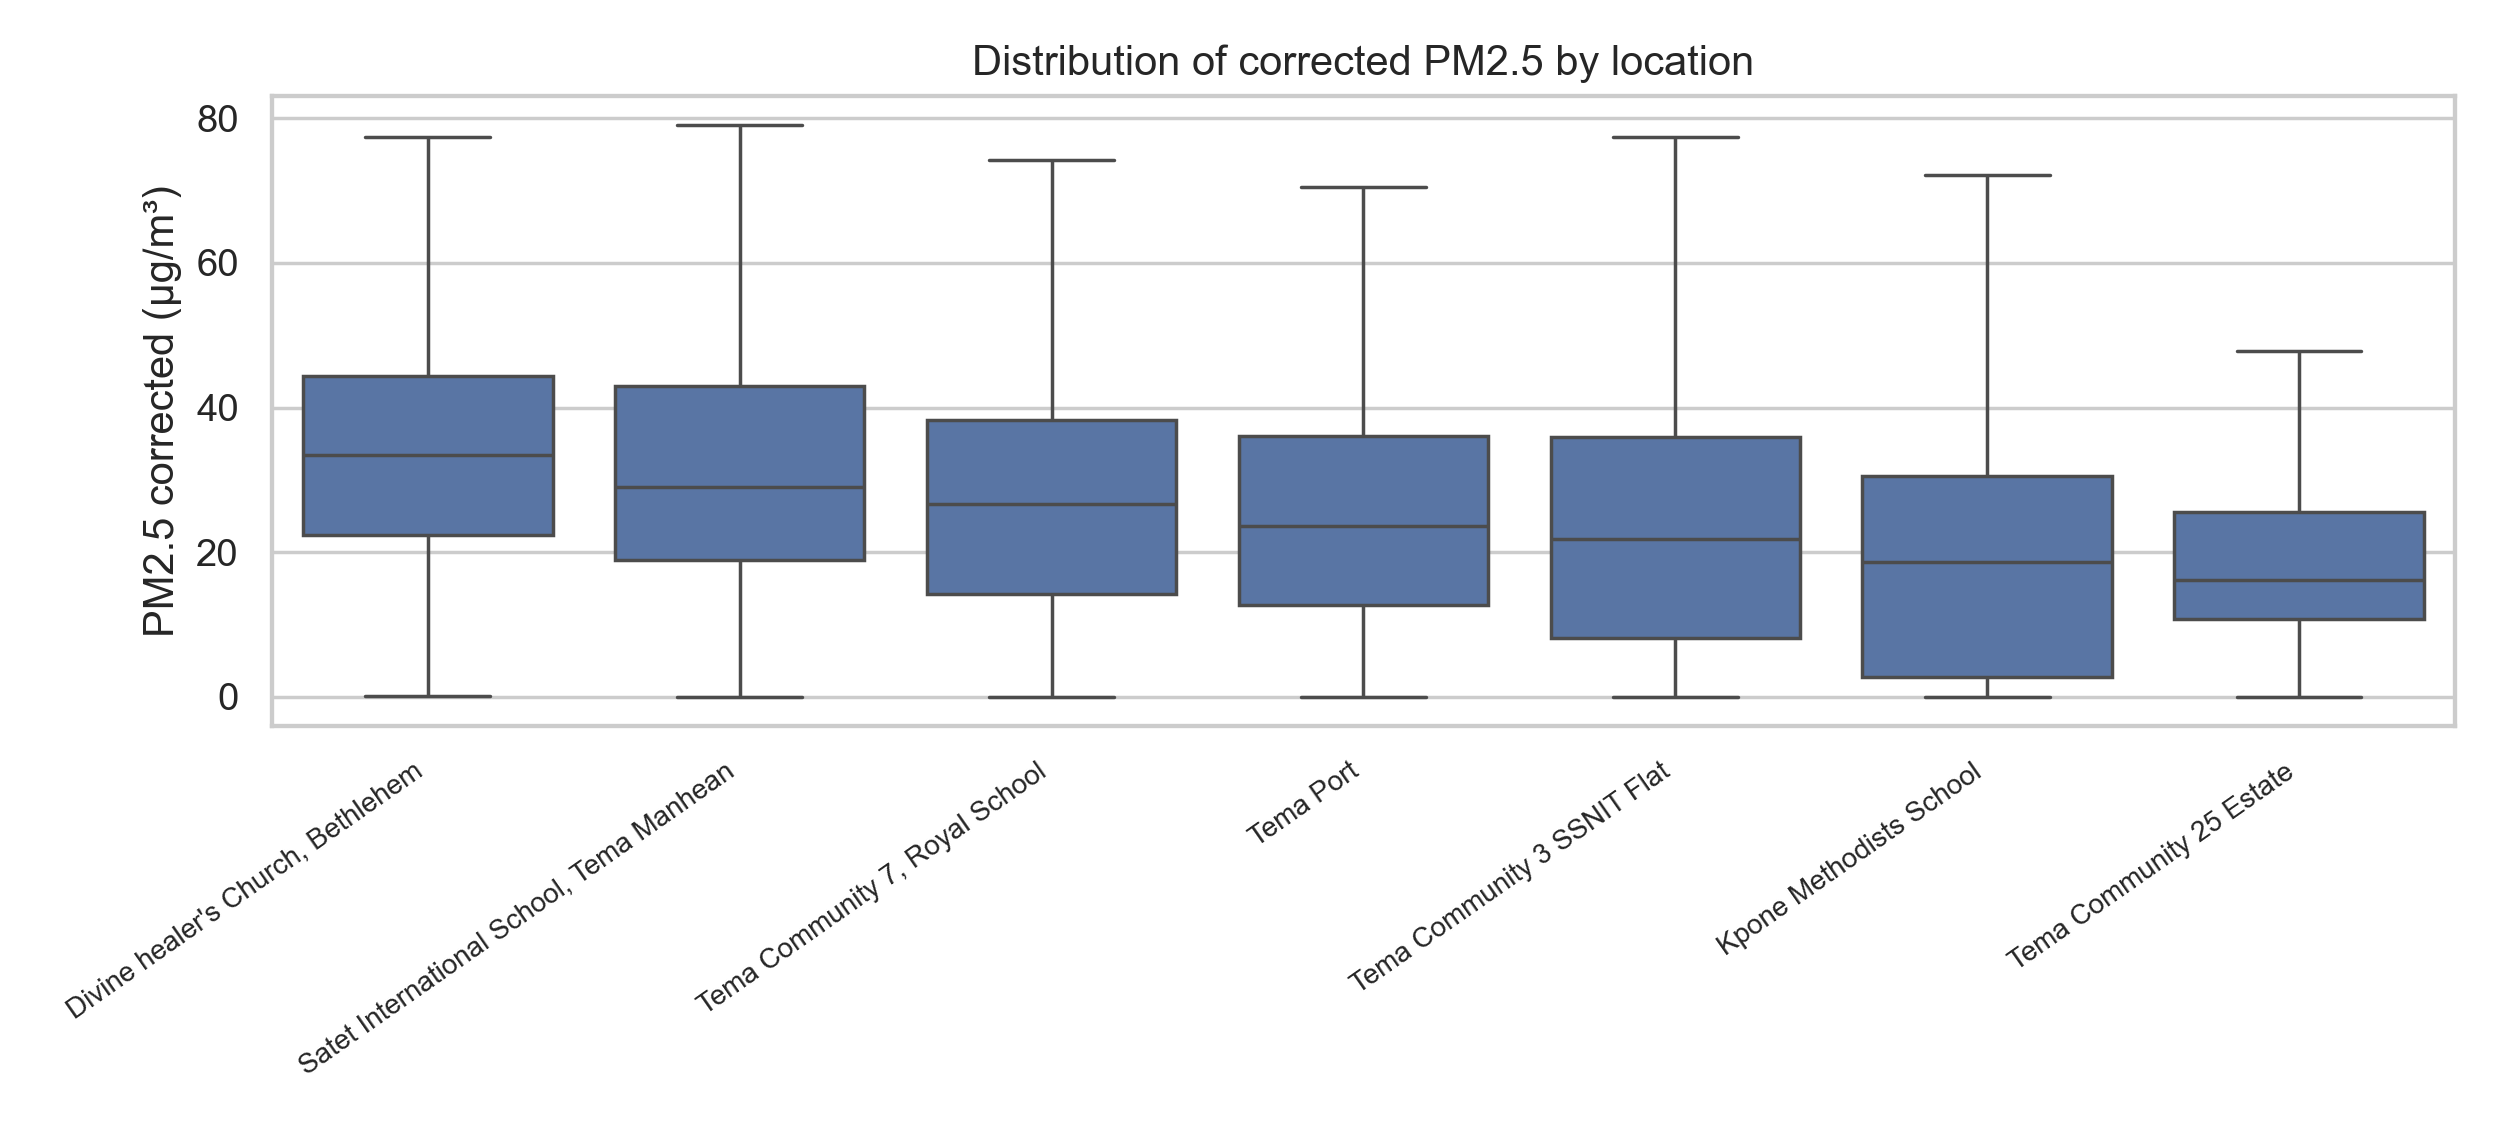
\includegraphics[width=0.92\textwidth]{eda_pm25_boxplot_by_location.png}%
    \caption{Distribution of raw and corrected PM$_{2.5}$ ($\mu$g/m$^3$) by monitoring location.}
    \label{fig:pm25_distribution}
\end{figure*}

\subsection{Temporal diurnal Variation in corrected PM$_{2.5}$ Concentrations}
Pooling all locations on local hourly time, corrected PM$_{2.5}$ exhibits a pronounced diurnal cycle (Figure~\ref{fig:diurnal_pooled}). Pooled hourly means rise toward a morning maximum around 05:00--07:00 (means up to approximately 48~$\mu$g/m$^3$ near 06:00), decline through midday, and reach an afternoon minimum around 13:00--14:00 (median near 15--17~$\mu$g/m$^3$), before increasing again through evening hours. This profile is broadly consistent with coupled influences of boundary-layer ventilation, emission activity rhythms, and regional aerosol transport.

Harmattan versus pre-Harmattan regimes further reshape the diurnal curve (Figure~\ref{fig:diurnal_regime}). Under Harmattan conditions, pooled median concentrations remain elevated throughout the day; for example, median PM$_{2.5}$ near midday is substantially higher than under pre-Harmattan conditions at comparable clock hours (Harmattan midday medians near 23--26~$\mu$g/m$^3$ versus about 8--12~$\mu$g/m$^3$ pre-Harmattan). Early-morning peaks are likewise amplified during Harmattan (median near 50~$\mu$g/m$^3$ around 06:00) compared with pre-Harmattan (median near 36~$\mu$g/m$^3$). Together, Figures~\ref{fig:diurnal_pooled}--\ref{fig:diurnal_regime} motivate reporting forecast performance under pooled conditions while interpreting limitations whenever models must generalise across sharply different atmospheric regimes.

\begin{figure*}[t]
    \centering
    \begin{subfigure}[t]{0.48\textwidth}
        \centering
        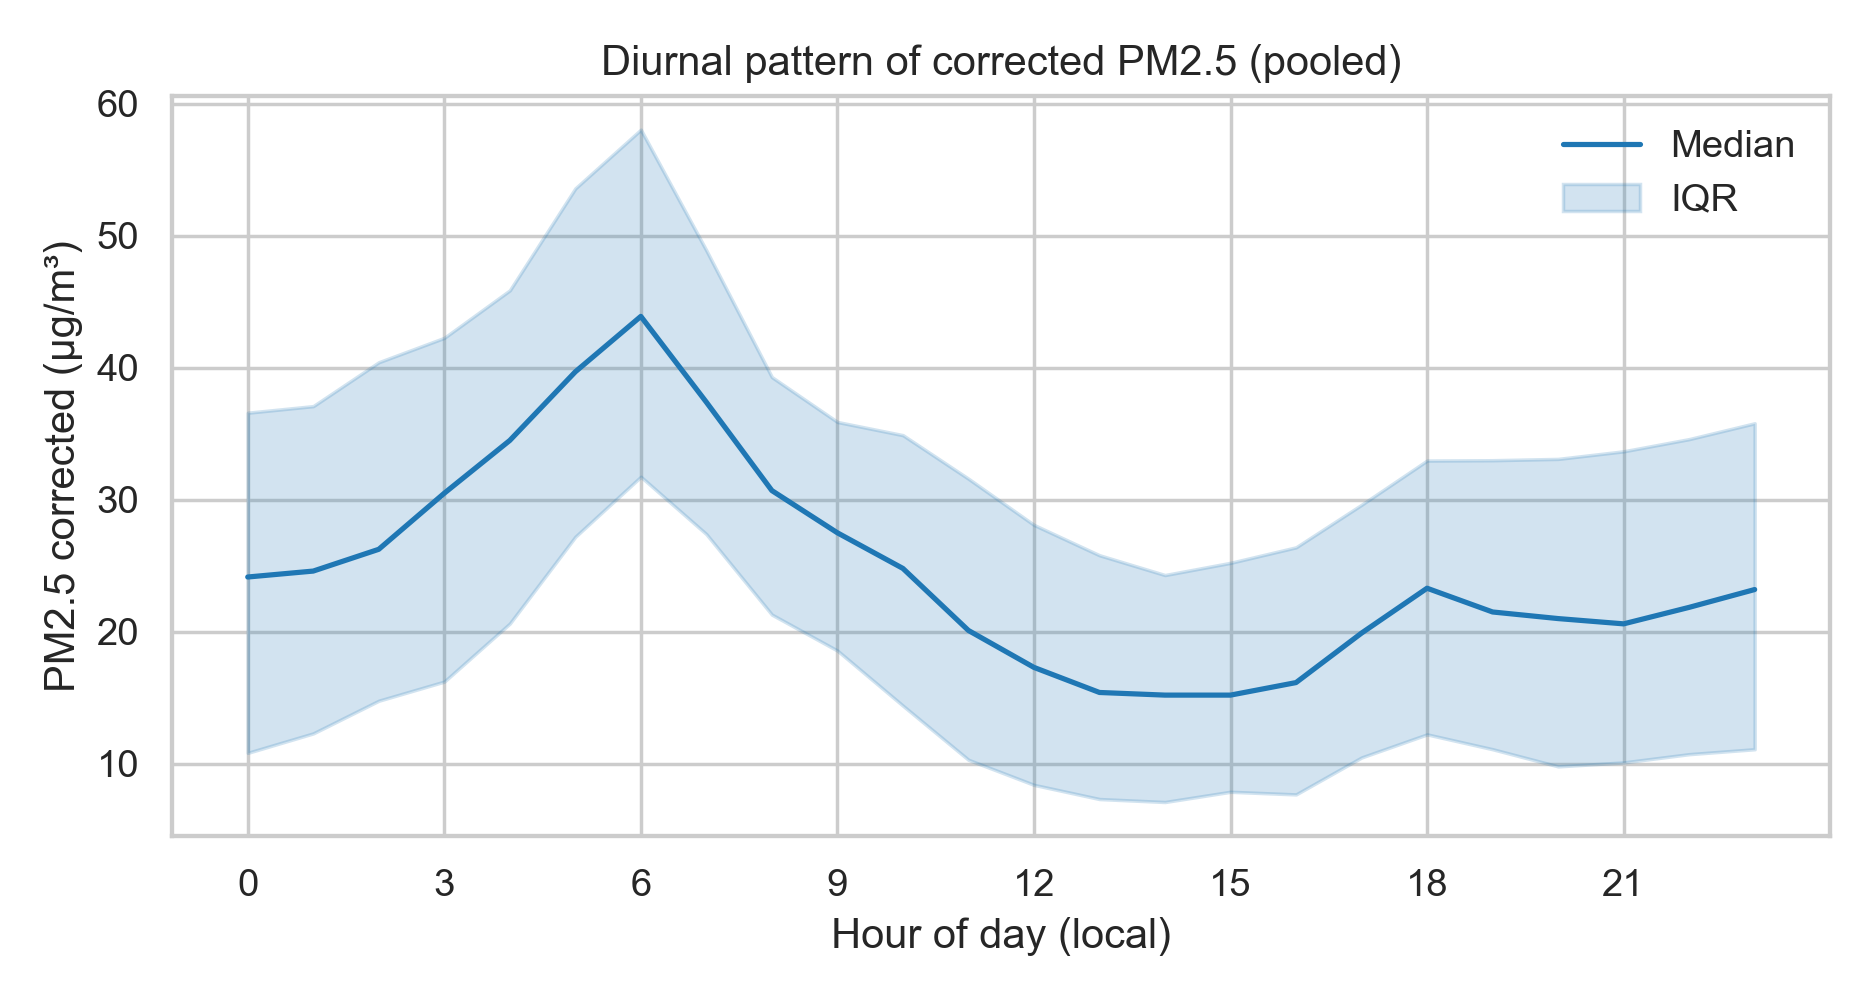
\includegraphics[width=\linewidth]{eda_diurnal_curve_pooled.png}%
        \caption{Pooled hourly profile (mean, median, and interquartile band).}%
        \label{fig:diurnal_pooled}
    \end{subfigure}\hfill
    \begin{subfigure}[t]{0.48\textwidth}
        \centering
        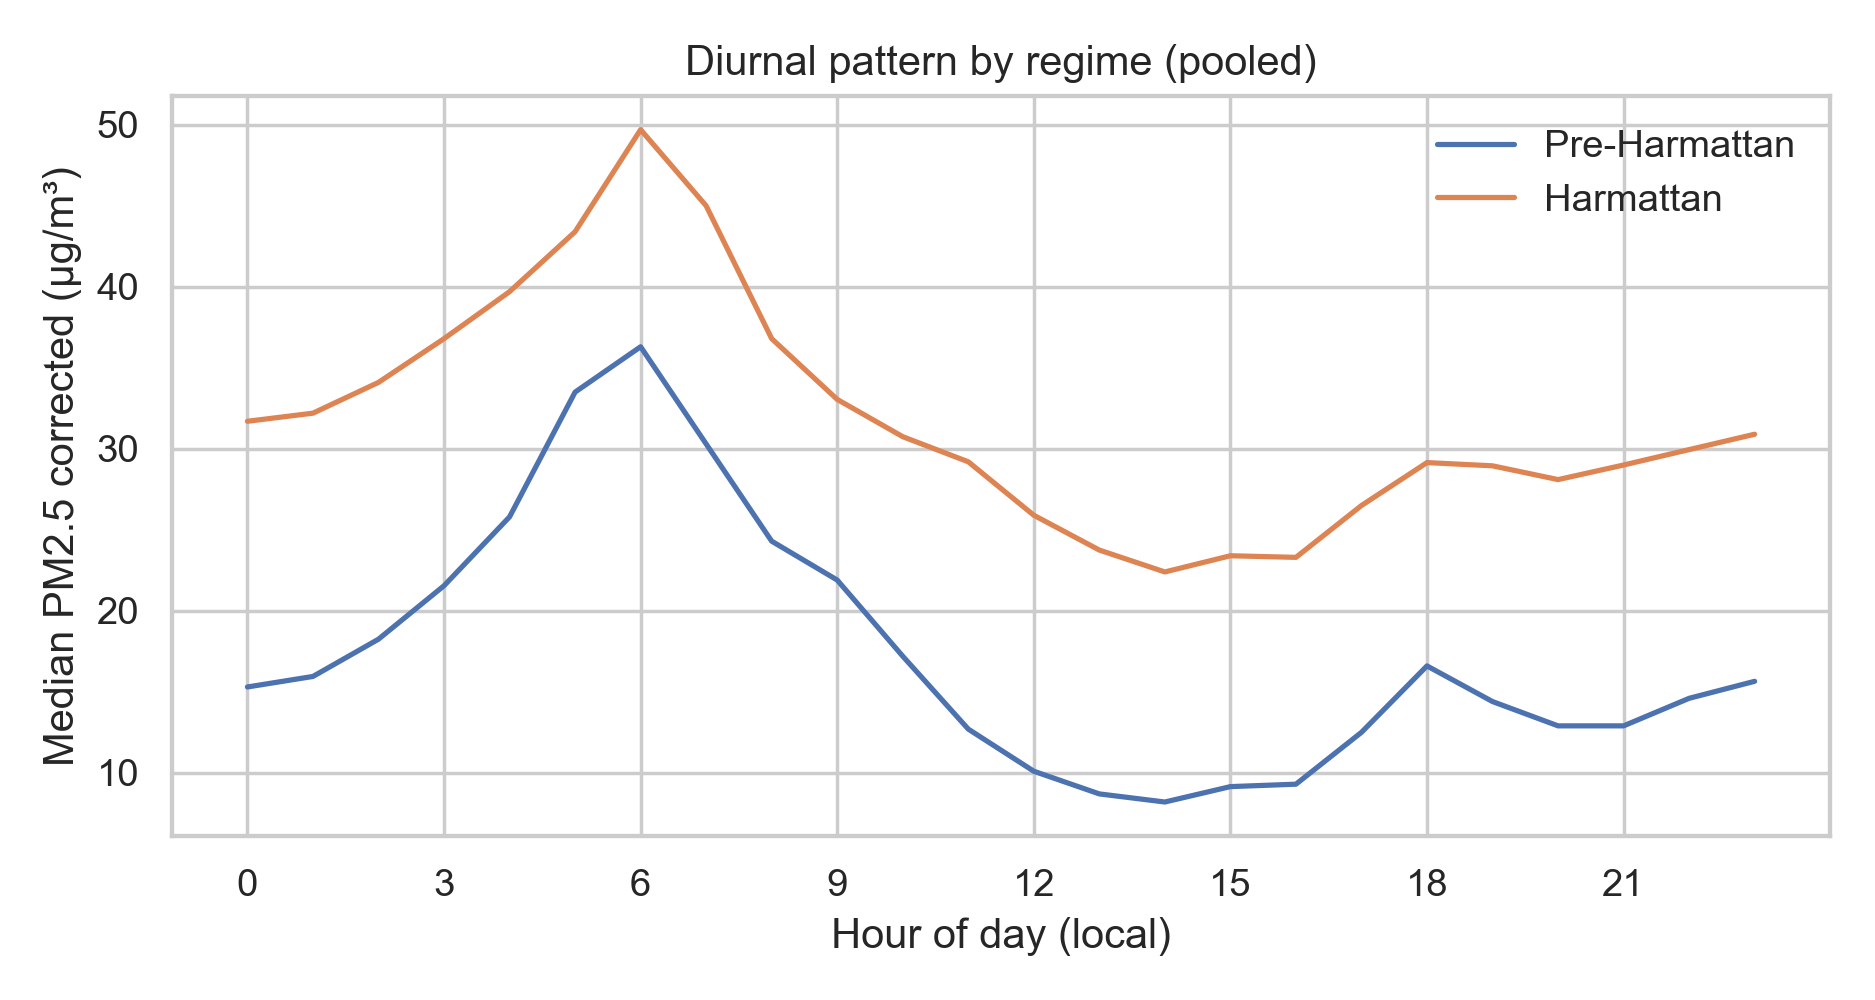
\includegraphics[width=\linewidth]{eda_diurnal_curve_by_regime.png}%
        \caption{Median diurnal curves stratified by Harmattan versus pre-Harmattan conditions.}%
        \label{fig:diurnal_regime}
    \end{subfigure}
    \caption{Diurnal variation in corrected PM$_{2.5}$ on local time (all sites pooled).}
    \label{fig:diurnal}
\end{figure*}

\subsection{Temporal Multi-Horizon predictions}
Forecasting models are trained and evaluated as \emph{direct} horizon-specific regressors on leakage-safe splits defined by label time (Section~\ref{sec2}), with horizons $H\in\{24,168,336,672\}$ hours.

Figure~\ref{fig:forecast_mae} summarises pooled test-set MAE across horizons for a compact set of interpretable benchmarks: both sequence architectures (LSTM and LSTM with multi-head attention), the restricted ridge autoregressive baseline with Fourier terms, seasonal naïve forecasting anchored at weekly recurrence, and---for context---linear SVR on engineered lag features. The chart makes two empirical features immediate: absolute error tends to rise with horizon for several baselines, while relative rankings reorganise at medium horizons where structured linear models become competitive.

\begin{figure*}[t]
    \centering
    
\includegraphics[width=0.92\textwidth]{results_mae_by_horizon.png}%
    \caption{Mean absolute error (MAE; $\mu$g/m$^3$) on pooled multi-site test windows for selected models, shown by direct forecasting horizon.}
    \label{fig:forecast_mae}
\end{figure*}

Table~\ref{tab:forecast-summary} complements Figure~\ref{fig:forecast_mae} with RMSE and $R^2$ alongside MAE for headline comparisons used in Sections~\ref{sec:res24}--\ref{sec:res672}. Episode-focused errors in the upper decile of observed concentrations remain materially larger than pooled MAE for deep models (not reproduced column-by-column here), reflecting the heavy upper tail documented in Section~3.1.

\begin{table}[H]
\centering
\caption{Representative out-of-sample forecasting accuracy on pooled multi-site test splits (corrected PM$_{2.5}$, $\mu$g/m$^3$). Sequence models use TensorFlow-backed Keras training; ``Ridge AR+Fourier'' denotes the restricted autoregressive ridge baseline with seasonal Fourier terms.}
\label{tab:forecast-summary}
\resizebox{0.95\textwidth}{!}{%
\begin{tabular}{llrrr}
\toprule
Horizon & Model & MAE & RMSE & $R^2$ \\
\midrule
24~h & LSTM + multi-head attention & 11.70 & 17.44 & 0.220 \\
24~h & Ridge AR+Fourier & 11.75 & 18.16 & 0.215 \\
24~h & Seasonal naïve (weekly anchor) & 14.59 & 21.46 & $-0.094$ \\
\midrule
7~d (168~h) & LSTM & 13.42 & 18.81 & 0.150 \\
7~d (168~h) & LSTM + multi-head attention & 13.67 & 19.43 & 0.093 \\
7~d (168~h) & Seasonal naïve (weekly anchor) & 15.39 & 22.74 & $-0.226$ \\
\midrule
14~d (336~h) & Linear SVR (tabular lags) & 13.94 & 19.06 & 0.136 \\
14~d (336~h) & LSTM & 14.46 & 20.61 & 0.135 \\
14~d (336~h) & LSTM + multi-head attention & 16.29 & 22.31 & $-0.014$ \\
\midrule
28~d (672~h) & LSTM + multi-head attention & 13.48 & 20.56 & $-0.126$ \\
28~d (672~h) & LSTM & 14.15 & 20.52 & $-0.122$ \\
28~d (672~h) & Ridge AR+Fourier & 15.28 & 20.92 & $-0.041$ \\
\bottomrule
\end{tabular}}
\end{table}

\begin{table}[H]
\centering
\caption{Forecast accuracy stratified by regime on a regime-spanning evaluation window (test window length increased to 84~days to include both pre-Harmattan and Harmattan periods). Values are MAE ($\mu$g/m$^3$) on the test set for simple benchmarks; this table is intended as a regime-aware diagnostic complementary to the primary 28-day test results in Table~\ref{tab:forecast-summary}.}
\label{tab:forecast-regime}
\resizebox{0.95\textwidth}{!}{%
\begin{tabular}{llrrr}
\toprule
Horizon & Model & Overall MAE & Pre-Harmattan MAE & Harmattan MAE \\
\midrule
24~h & Naïve level (persistence) & 12.59 & 10.40 & 12.84 \\
24~h & Seasonal naïve (weekly anchor) & 13.75 & 10.86 & 14.10 \\
\midrule
7~d (168~h) & Naïve level (persistence) & 13.61 & 10.84 & 14.25 \\
7~d (168~h) & Seasonal naïve (weekly anchor) & 14.46 & 13.31 & 14.73 \\
\bottomrule
\end{tabular}}
\end{table}

\subsubsection{Short-term (24hr)}\label{sec:res24}
At $H=24$~h, the attention-augmented sequence model attains the lowest MAE among the headline comparisons in Table~\ref{tab:forecast-summary} (MAE~=~11.70~$\mu$g/m$^3$; RMSE~=~17.44~$\mu$g/m$^3$; $R^2\approx 0.22$), narrowly edging the ridge AR+Fourier baseline (MAE~=~11.75~$\mu$g/m$^3$). Relative to the weekly seasonal naïve benchmark shown in the table, MAE falls by roughly 2--3~$\mu$g/m$^3$, indicating that learned nonlinear dynamics provide measurable short-horizon value beyond simple seasonal anchors on this evaluation window.

\subsubsection{Mid-terms (7d and 14d)}\label{sec:res714}
For $H=168$~h, sequence models outperform the weekly seasonal naïve comparator by a clear margin on MAE (Table~\ref{tab:forecast-summary}; Figure~\ref{fig:forecast_mae}). Vanilla LSTM slightly improves upon LSTM+attention on MAE at this horizon (13.42 vs.\ 13.67~$\mu$g/m$^3$), illustrating that attention is not guaranteed to reduce point error at weekly lead times without additional tuning.

At $H=336$~h, rankings diversify: linear SVR on tabular lag features achieves the lowest MAE among the tabulated candidates (13.94~$\mu$g/m$^3$), marginally ahead of LSTM (14.46~$\mu$g/m$^3$). LSTM+attention records higher MAE (16.29~$\mu$g/m$^3$) and near-zero pooled explanatory skill ($R^2\approx -0.01$). Rather than interpreting this as evidence against sequence modelling broadly, we emphasise that medium-horizon forecasting here approaches the limits of pooled stationarity assumptions under regime mixing; reporting should therefore pair accuracy metrics with regime-aware diagnostics whenever possible.

\subsubsection{Long-terms (28d)}\label{sec:res672}
At $H=672$~h, pooled $R^2$ for the sequence models tabulated becomes negative (Table~\ref{tab:forecast-summary}), indicating limited incremental variance explained relative to the test-set mean predictor under this split. Nonetheless, MAE remains competitive for operational comparisons: LSTM+attention yields MAE~=~13.48~$\mu$g/m$^3$, slightly lower than LSTM (14.15~$\mu$g/m$^3$) and ridge AR+Fourier (15.28~$\mu$g/m$^3$). Upper-tail episodes remain systematically harder for all models at long leads, consistent with the concentration extremes visible in Figure~\ref{fig:pm25_distribution}.

\section{Discussion}\label{sec4}

\section{Conclusion}\label{sec5}



\printcredits

%% Loading bibliography style file
% \bibliographystyle{model1-num-names}
\bibliographystyle{cas-model2-names}

% Loading bibliography database
\bibliography{cas-refs}


%\vskip3pt

% \bio{}
% Author biography without author photo.
% Author biography. Author biography. Author biography.
% Author biography. Author biography. Author biography.
% Author biography. Author biography. Author biography.
% Author biography. Author biography. Author biography.
% Author biography. Author biography. Author biography.
% Author biography. Author biography. Author biography.
% Author biography. Author biography. Author biography.
% Author biography. Author biography. Author biography.
% Author biography. Author biography. Author biography.
% \endbio

% \bio{figs/pic1}
% Author biography with author photo.
% Author biography. Author biography. Author biography.
% Author biography. Author biography. Author biography.
% Author biography. Author biography. Author biography.
% Author biography. Author biography. Author biography.
% Author biography. Author biography. Author biography.
% Author biography. Author biography. Author biography.
% Author biography. Author biography. Author biography.
% Author biography. Author biography. Author biography.
% Author biography. Author biography. Author biography.
% \endbio

% \bio{figs/pic1}
% Author biography with author photo.
% Author biography. Author biography. Author biography.
% Author biography. Author biography. Author biography.
% Author biography. Author biography. Author biography.
% Author biography. Author biography. Author biography.
% \endbio

\end{document}

